\documentclass[border=2pt]{standalone}
\usepackage{pgfplots}
\pgfplotsset{compat=1.18}
\begin{document}
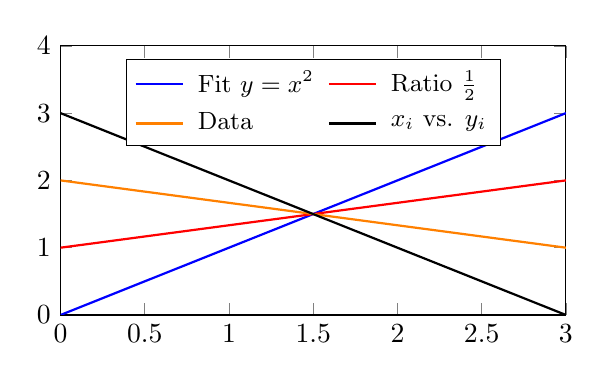
\begin{tikzpicture}
\begin{axis}[width=8cm,height=5cm,xmin=0,xmax=3,ymin=0,ymax=4,
  legend style={at={(.5,.95)},anchor=north,legend columns=2,
    column sep=3pt,row sep=2pt,font=\small},legend cell align=left]
  \addplot[blue,thick,mark=none] coordinates {(0,0)(3,3)};
  \addlegendentry{Fit $y=x^2$}
  \addplot[red,thick,mark=none] coordinates {(0,1)(3,2)};
  \addlegendentry{Ratio $\frac{1}{2}$}
  \addplot[orange,thick,mark=none] coordinates {(0,2)(3,1)};
  \addlegendentry{Data}
  \addplot[black,thick,mark=none] coordinates {(0,3)(3,0)};
  \addlegendentry{$x_i$ vs. $y_i$}
\end{axis}
\end{tikzpicture}
\end{document}
